\chapter{Niching Algorithms}
\label{niching}
\section{Background}
Aerodynamic shape optimization (ASO) is defined as finding the shape that optimizes a performance quantity subject to drag, geometrical constraints. Much of the work carried out in the past involved finding the single best optimum solution. However, during the design process, identifying other optimal designs may positively impact the cost and performance. Many aerodynamics optimization problems can be unimodal or multimodal. The parallel niching optimization algorithms direct the given multimodal optimization problem to identify the multiple optima in the given design space. This chapter contains a detailed explanation of the DE based parallel niching algorithms.

Differential evolution (DE) algorithm deals with finding the best result for a given objective function. However, this is normal when the problem is of type Unconstrained Numerical Optimization problems (UNOPs). If the objective function possesses the constraints (equality or inequality) generally called as Constrained Numerical Optimization problems (CNOPs), then DE is not designed to handle the constraint and which limits its scope to UNOPs. To solve the CNOPs, a modification to the DE algorithm at some stage in its hierarchy is necessary.

 Furthermore, the DE generally results in a global optimum, which again limits its scope to a problem where finding a global optimum is prior important. In case of problems where finding multiple good solutions is important rather than the best solution, a modification to the DE algorithm is necessary. These modifications will help obtain multiple optimum values (good results), also called as \textbf{multimodal optimization problem}. These modifications to the DE algorithm results in \textbf{Niching Algorithms}. These techniques will enhance the population’s diversity by locating the optimal solution that lies in different parts of the search space. A considerable amount of research has taken place in constraint handling and multimodal optimization using a nature-inspired algorithm. Upcoming sections contain a detailed explanation  on DE and the modification to algorithms.
\section{Differential Evolution}
DE is a population-based optimization algorithm, where operators for mutation, crossover, and selection act to create a new population from an existing one. Eventually, through a series of iterations, the population will converge on to a globally optimal solution \cite{Poole3}. The DE is suitable for problems with discontinuous objectives, also with a problem having multiple local optima (multimodality). However, DE has slow convergence. Nearly 200 times more functional evaluations are required for Gradient-free methods as compared to gradient-based methods \cite{oleg}.

The DE is a parallel direct search method which utilizes $N$
D-dimensional design vectors \textbf{x$_{n,G}$}, where n = 1, 2, ... , N and g is the generation ranging between $[1, G]$. $N$ does not alter during the optimization
process. The initial population is chosen randomly and should cover the entire design space. As a rule, it is assumed to follow a uniform probability distribution for all random decisions unless otherwise stated. In case a preliminary solution is available, the initial population might be generated by adding normal distributed random deviations to the nominal solution $\textbf{x}_{nom,0}$. The DE generates another vectors by adding the weighted difference between two population vectors to a third vector. This operation is called \textit{mutation}.

The mutated vector individuals are merged with the individuals of another predetermined vector, the target vector, to generate the \textit{trial vector}. This operation is referred to as "\textit{crossover}." If the trial vector yields a lower cost function value than the target vector, the trial vector replaces the target vector in the following generation. This last operation is called "\textit{selection}". Each population vector has to serve once as the target vector so that $ N $ competitions occur in a given generation \cite{storn}.

The mathematical representation of the DE algorithm is explained as follows.
\begin{enumerate}
\item \underline{Initialization}: Here the initial population $N$ is generated randomly as: 
\begin{equation}
\textbf{x}_{n,g}^{d}=\textbf{L}^{d}+\operatorname{rand}(0,1)\left(\textbf{U}^{d}-\textbf{L}^{d}\right)
\label{initlize}
\end{equation}
where $rand(0, 1)$ is a uniformly distributed random number on the interval [0, 1]. $L^d$ and $U^d$ represents the lower and the upper limits of the design space respectively. And, $d$ is dimension of problem which can be $(d\in\{1, \ldots, D\}))$.

\item \underline{Mutation}: For each individual in the population, corresponding donor vector is generated as follows: initially, the weighted difference is taken between two randomly selected individuals from population,then it is added it to base vector (\textbf{x}$_{b,G}$). There are several strategies proposed that define the base vector. If in case DE/best/1 strategy is chosen, then the \(n\)-th donor vector is represented using equation \ref{best_mutation}. 
\begin{equation}
\mathbf{v}_{n}=\mathbf{x}_{b}(t)+F\left(\mathbf{x}_{r_{1}}(t)-\mathbf{x}_{r_{2}}(t)\right)
\label{best_mutation}
\end{equation}
$$
b=\underset{i \in\{1, \ldots, N\}}{\arg \min } f\left(\mathbf{x}_{i}\right)
$$
where, $F$ is the scaling factor ranging between [0, 1]. A higher scaling factor may force the donor individual to fall out of design space. Whereas, the lower value will generate the donor vector close to target individual. A value of $F = 0.5$ is considered to be a good trade off. $x_{b,g-1}$ is the best individual from the previous generation. $r_1$ and $r_2$ are uniformly distributed random integers in the interval [1, N] such that \(r_{1} \neq r_{2} \neq b\) and \(r_{1} \neq r_{2} \neq n\). A better representation of mutation stage in 2-D design space is shown in figure \ref{mutation}.
\begin{figure}[!ht]
    \centering
    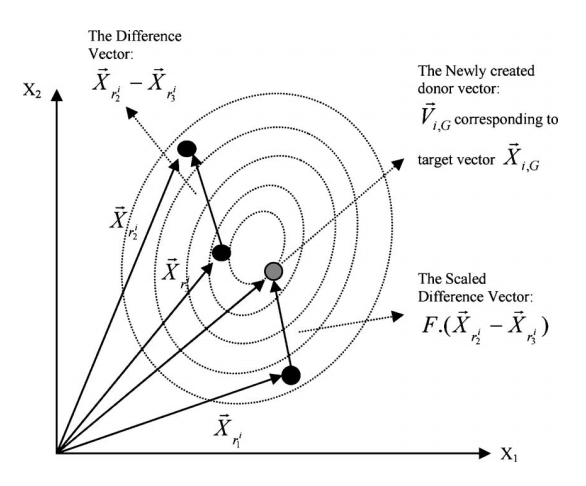
\includegraphics[scale = 0.5]{figures/mutation.png}
    \caption{2-D design space representing mutation stage \cite{storn}.}
    \label{mutation}
\end{figure}

\item \underline{Cross-over}: In this stage, elements from the target vector and donor vector are combined in a specific order to get a trial vector (\textbf{u}$_{n,g}$). This process is referred as binomial crossover. This stage play a vital role in increasing the population's diversity, and is shown in equation \ref{cross-over}.

\begin{figure}[!ht]
    \centering
    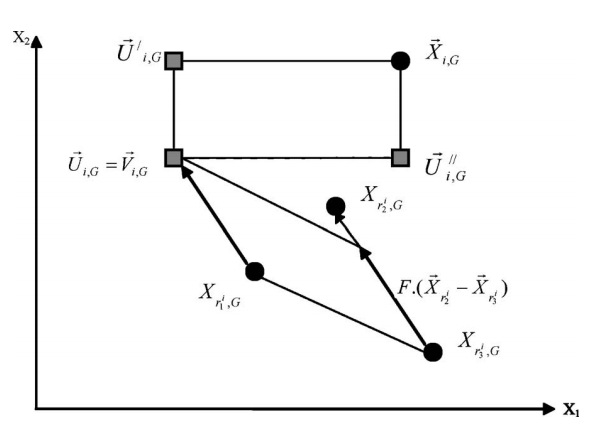
\includegraphics[scale = 0.5]{figures/crossover.png}
    \caption{Different possible trial vector formed due to Uniform/Binomial crossover between mutant vector and target vector in 2-D design space\cite{storn}.}
    \label{crossover}
\end{figure}

\begin{equation}
\mathbf{u}_{n,g}=\left\{\begin{array}{ll}{\mathbf{v}_{n,g}} & {\text { if rand }(0,1) \leq C R \text { or } r_{n}=d} \\ {\mathbf{x}_{n,g}} & {\text { otherwise }}\end{array}\right.
\label{cross-over}
\end{equation}
where $r_n$ is the uniformly distributed random integer in the interval [1, D], and $CR$ is the crossover probability. $CR = 1$ implies there is no diversity, meaning the parent individuals are not carried to the next generation. On the other hand, $CR = 0$ implies that all generated elements are the same as parent elements, so there is no evolution over generations.

\item \underline{Selection}: The trial individuals and target individuals are compared based on their function values. During the problem with the minimization case, an individual with minimum function value is retained. On the other hand, for maximization problems, an individual with a maximum function value is retained. Equation \ref{selection} represents the selection phase.
\begin{equation}
\mathbf{x}_{n}(t+1)=\left\{\begin{array}{ll}{\mathbf{u}_{n}} & {\text { if } f\left(\mathbf{u}_{n}\right) \leq f\left(\mathbf{x}_{n}(t)\right)} \\ {\mathbf{x}_{n}(t)} & {\text { otherwise }}\end{array}\right.
\label{selection}
\end{equation}

\item \underline{Stopping condition}: The optimization can have single or multiple stopping conditions, like the maximum number of function evaluations, epsilon value, to name a few. The author D.J.Poole used the maximum number of function evaluations ($FEs_{max}$) as the stopping condition for all the algorithms.
\end{enumerate}

The algorithm \ref{DE algorithm} depicts the pseudo-code for the DE algorithm.
\begin{algorithm}[!ht]
\SetAlgoNoLine
 Randomly initialise individuals and calculate objective\\
 \While{\text { $FEs <FEs_{max}$ }}
 {
  \For{$n=1 \rightarrow N$}
  {
  Perform mutation: equation \ref{best_mutation}\\
  Perform binomial crossover: equation \ref{cross-over}\\
  Calculate objective and constraints of trial vector
  }
  \For{$n=1 \rightarrow N$}{
 Update $n$-th target vector: equation \ref{selection}
 }
 }
 \caption{DE algorithm}
 \label{DE algorithm}
\end{algorithm}

In the next section, details about mutation strategies are explained. 

\section{DE Strategies}
In the DE algorithm, there are different variants for the mutation stage. Some of these are mentioned in the upcoming subsections \cite{chi}.

\subsection{DE/rand/1}
In this strategy, the mutation stage is carried out by taking single pair of the weighted difference. The individuals involved are randomly selected from the populations, Further, the weighted difference is added to base individual resulting in target vector as shown in equation \ref{DE-rand-1}.
\begin{equation}
    \mathbf{v}_{n, g}=\mathbf{x}_{r_{1}, g}+F.\left(\mathbf{x}_{r_{2}, g}-\mathbf{x}_{r_{3}, g}\right)
    \label{DE-rand-1}
\end{equation}

\subsection{DE/best/1}
This method work the same way as DE/rand/1 strategy, except that it generates the individual base vector $x_{b}$ as in equation \ref{DE-best-1}.
\begin{equation}
    \mathbf{v}_{n, g}=\mathbf{x}_{b, g-1}+F.\left(\mathbf{x}_{r_{1}, g}-\mathbf{x}_{r_{2}, g}\right)
    \label{DE-best-1}
\end{equation}
where,
$$
b=\underset{i \in\{1, \ldots, N\}}{\arg \min } f\left(\mathbf{x}_{i, g-1}\right)
$$

\subsection{DE/best/2}
This strategy involve evaluating the mutant vector with two weighted ($F_1, F_2$) differences of vectors which are picked randomly from the population size \(N\), and added to base vector (best) \(x_b\). Equation \ref{DE-best-2} represents the same.
\begin{equation}
  \mathbf{v}_{n, g}=\mathbf{x}_{b, g-1}
+F_{1}.\left(\mathbf{x}_{r_{1}, g}-\mathbf{x}_{r_{2}, g}\right)
+F_{2}.\left(\mathbf{x}_{r_{3}, g}-\mathbf{x}_{r_{4}, g}\right)
\label{DE-best-2}
\end{equation}
where,
$$
b=\underset{i \in\{1, \ldots, N\}}{\arg \min } f\left(\mathbf{x}_{i, g}\right)
$$

\subsection{DE/current to best/2}
In this strategy, one of the two weighted differences will take place between the best vector and the vector index for which perturbation is carried out. Equation \ref{DE-ctob-2} depicts the above strategy. 
$$\mathbf{v}_{n}=\mathbf{x}_{b}(t)
+F_{1}\left(\mathbf{x}_{r_{1}}(t)-\mathbf{x}_{r_{2}}(t)\right)
+F_{2}\left(\mathbf{x}_{b}(t)-\mathbf{x}_{r_n}(t)\right)$$
where,
$$
b=\underset{i \in\{1, \ldots, N\}}{\arg \min } f\left(\mathbf{x}_{i}\right)
$$

\subsection{DE/rand/2}
This strategy involve two weighted differences between individuals. These individuals are randomly selected in the given population. Equation \ref{DE-rand-2} represents the mutant vector generation using the DE/rand/2 strategy. 
$$\mathbf{v}_{n}=\mathbf{x}_{r_{1}}(t)
+F_{1}\left(\mathbf{x}_{r_{2}}(t)-\mathbf{x}_{r_{3}}(t)\right)
+F_{2}\left(\mathbf{x}_{r_{4}}(t)-\mathbf{x}_{r_{5}}(t)\right)$$
where, $r_1, r_2, r_3, r_4, r_5 \in [1, NP]$ and $\neq$ running index $i$. 


\subsection{Comparision between strategies}
The author H.Chi \cite{chi} mention that the strategies like \textit{DE/best/1}, \textit{DE/best/2} and \textit{DE/current to best/2} can improve the convergence rate of DE, and converge in the local optimal due to usage of the best vector. On the other hand, \textit{DE/rand/2} and \textit{DE/rand/1} relatively enhance the convergence rate of finding the global optimal but have slow convergence speed. Several test functions like Sphere function, Rosenbock's function, Step function, Quartic function, etc. are tested using the Niching algorithm, and results obtained coincide with the actual optimal values. Chapter \ref{results} highlights more on test function results.

\section{Constraint handling}
The feasibility rules published by Deb \cite{Daniel} assist in handling the constraints to the problems. The rules are as stated: when choosing between two
locations, if both locations are feasible, the one with the best fitness value wins. If a single location is feasible, then select the same. Otherwise, select the location with the least constraint violations. Mathematically, using domination operator, where, given two locations $x_a$ and $x_b$, $x_b$ dominates $x_a$ based on the following:
\begin{equation}
\mathbf{x}_{a} \prec \mathbf{x}_{b}
\Leftrightarrow\left\{
\begin{array}{ll}
{f\left(\mathbf{x}_{b}\right)<f\left(\mathbf{x}_{a}\right)} & {\text { and } \quad \phi\left(\mathbf{x}_{a}\right), \phi\left(\mathbf{x}_{b}\right)=0} \\
{\phi\left(\mathbf{x}_{b}\right)=0} & {\text { and } \quad \phi\left(\mathbf{x}_{a}\right)>0} \\
{\phi\left(\mathbf{x}_{b}\right)<\phi\left(\mathbf{x}_{a}\right)} & {\text { and } \quad \phi\left(\mathbf{x}_{a}\right), \phi\left(\mathbf{x}_{b}\right)>0}
\end{array}\right.
\label{feas}
\end{equation}

where $\phi$ is the constraint violation given by:

\begin{equation}
\phi (\mathbf{x})=\sum_{i=1}^{p} \max \left[0, g_{i}(\mathbf{x})\right]+\sum_{j=1}^{q}\left|h_{j}(\mathbf{x})\right|
\end{equation}

In DE, these feasibility rules are commonly used in the selection step to determine whether the trial vector should
replace the target vector. Hence at selection stage:

\begin{equation}
\mathbf{x}_{n}(t+1)=\left\{\begin{array}{ll}{\mathbf{u}_{n}} & {\text { if } \mathbf{x}_{n}(t) \prec \mathbf{u}_{n}} \\ {\mathbf{x}_{n}(t)} & {\text { otherwise }}\end{array}\right.
\label{selection_constraint}
\end{equation}

\section{Control variable}

There are a few parameters that decide the algorithm progress towards the optimal points. The NP, F, and CR are the important parameters in the DE algorithm. D.J.Poole\cite{storn} states that it is not difficult to guess the range of values for these algorithms. According to the author, NP is to be between 5D and 10D. A value of F = 0.5 is usually the right choice. Furthermore, for CR probability, a value of 0.1 would work fine. However, the higher the value of CR faster will be the convergence. So it always the right choice to test the algorithm with a CR value of 0.9.

\section{Parallel and Sequential decomposition}
There are two ways to implement the algorithm, sequential flow, and parallel flow. Taking DE into consideration, the sequential form of DE constitutes the mutation, crossover, and selection phases in sequential order. For each population within a design space, all these phases are carried out in sequential order, as shown in fig[\ref{sequential_form_algo}]. However, this will result in an inefficient implementation. Instead, a parallel form of implementation can be followed. Here, the entire population is subjected to mutation, crossover, selection phases at once. Then, the comparison between the populations is carried out later. 

The most expensive part of the aerodynamic optimization problem is objective function evaluation, which is CFD evaluation. In the case of solving the above problem, the parallel decomposition of algorithm wins over the sequential. Also, each of the population can be thread into single processing resulting in parallel computation of the CFD simulations as shown in fig \ref{parallel_form_algo}. The pictorial representation of both parallel and sequential decomposition of the algorithm is as shown below,
\begin{figure}[!ht]
    \centering
    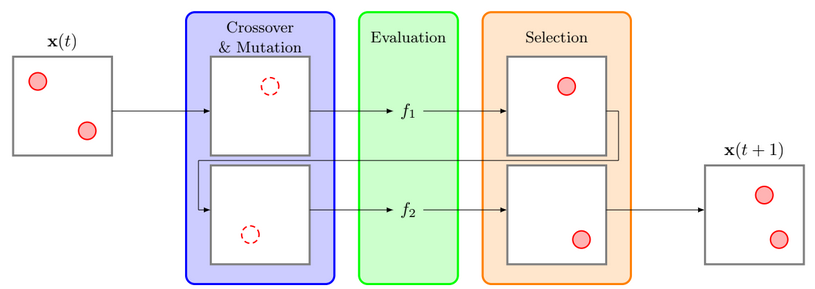
\includegraphics[scale = 0.5]{figures/sequential_form_DE.png}
    \caption{Sequential decomposition of algorithm\cite{Poole2}.}
    \label{sequential_form_algo}
\end{figure}

\begin{figure}[!ht]
    \centering
    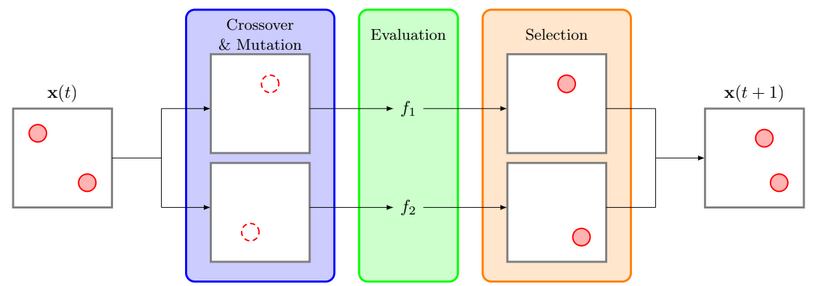
\includegraphics[scale = 0.5]{figures/parallel_form_DE.png}
    \caption{Parallel decomposition of algorithm\cite{Poole2}.}
    \label{parallel_form_algo}
\end{figure}

\section{Sequential Niching algorithm}
As mentioned before, there are two ways to implement the DE algorithm. The upcoming subsections explain different sequential niching algorithms. Among these, few of the niching algorithms are recreated in python and implemented on test functions like Ackley function, Rastrigin function, and Egg holder function. The result coincides with the one published by the author and is discussed in chapter \ref{results}. 

The algorithm involved in aerospace optimization generally follows the population crowding technique\cite{De_jong,thomsen}, fitness sharing\cite{michigan,thomsen,goldberg}, clearing\cite{petrowski}, speciation\cite{balazs,Li}, local neighborhoods\cite{vrahatis,vrahatis_1}, to name a few. Li $et$ $al$. present a full review of these properties\cite{li_1}. Following are few of the sequential niching algorithms which are implemented in python and as follows\cite{Poole3}, 
$$
\begin{array}{l}
{\bullet \text { Feasible DE }(\mathrm{fDE}), \text { which is based on canonical DE, }} \\ 
{\bullet \text { Feasible DE using nrandl mutation (fNRAND1), }}\\
{\bullet \text { Feasible DE using inrand } 1 / r \text { (nearest neighbour with ring network) mutation (fINRAND1), }} \\
{\bullet \text { Feasible crowding DE (fCDE), which is based on the CDE algorithm, }} \\
{\bullet \text { Feasible neighbourhood-based CDE (fNCDE), which is based on the NCDE algorithm,  }} \\ {\bullet \text { Feasible species-based DE (fSDE), which is based on the SDE algorithm, }} \\
{\bullet \text { Feasible neighbourhood-based SDE (fNSDE), which is based on the NSDE algorithm, }} \\ {\bullet \text { Feasible fitness-sharing DE (fSHDE), which is based on the SHDE algorithm, }}
\end{array}
$$


\subsection{fDE}
In this algorithm the selection stage is modified as stated by Deb and Saha\cite{Deb}, which uses equation [\ref{selection_constraint}]. further in the mutation stage, algorithm follows $rand/1/bin$ strategy.
\begin{algorithm}[!ht]
\SetAlgoNoLine
 Randomly initialise individuals and calculate objective\\
 \While{\text { $FEs <FEs_{max}$ }}
 {
  \For{$n=1 \rightarrow N$}
  {
  Perform rand/1 mutation: equation \ref{best_mutation}\\
  Perform binomial crossover: equation \ref{cross-over}\\
  Calculate objective and constraints of trial vector
  }
  \For{$n=1 \rightarrow N$}{
 Update $n$-th target vector: equation \ref{selection_constraint}
 }
 }
 \caption{fDE algorithm}
 \label{fDE algorithm}
\end{algorithm}

\subsection{fNRAND1}
In this algorithm, mutation stage is modified by taking the target vector of the \(n\)-th individual's nearest neighbour $x_{{NN}_n}$ as the base vector as shown. selection stage uses equation [\ref{selection_constraint}] as feasibility check.
\begin{equation}
\mathbf{v}_{n, g}=\mathbf{x}_{N N_{n, g}}+F.\left(\mathbf{x}_{r_{1}, g}-\mathbf{x}_{r_{2}, g}\right)
\label{fNRNAD1_equation}
\end{equation}
where,
$$N N_{n, g}=\underset{i \in\{1, \ldots, N\}, i \neq n} {\arg \min} \left\|\mathbf{x}_{n, g}-\mathbf{x}_{i, g}\right\|_{2}$$

\begin{algorithm}[!ht]
\SetAlgoNoLine
 Randomly initialise individuals and calculate objective\\
 \While{\text { $FEs <FEs_{max}$ }}
 {
  \For{$n=1 \rightarrow N$}
  {
  Find the nearest neighbour to $x_n$\\
  Perform nrand/1 mutation: equation \ref{fNRNAD1_equation}\\
  Perform binomial crossover: equation \ref{cross-over}\\
  Calculate objective and constraints of trial vector
  }
  \For{$n=1 \rightarrow N$}{
 Update $n$-th target vector: equation \ref{selection_constraint}
 }
 }
 \caption{fNRAND1 algorithm}
 \label{fNRAND1 algorithm}
\end{algorithm}

\subsection{fINRAND1}
This algorithm work similarly to the above mentioned, however in the mutation stage, the algorithm uses the target vector of the \(n\)-th individual’s nearest neighbor within its local neighborhood, $x_{INN_n}$, as the base vectors. Since it uses an index-based ring neighborhood, this algorithm reduces the computational complexity against the fNRAND1 algorithm.
\begin{equation}
\mathbf{v}_{n, g}=\mathbf{x}_{I N N_{n, g}}+F.\left(\mathbf{x}_{r_{1}, g}-\mathbf{x}_{r_{2}, g}\right)
\label{fINRAND1_equation}
\end{equation}
where,

$$
I N N_{n, g}=\left\{
\begin{array}{ll}
{\underset{i \in\{N, 2\}}{\arg \min} \left\|\mathbf{x}_{n, g}-\mathbf{x}_{i, g}\right\|_{2}} & {\text { if } n=1} \\
{\underset{i \in\{N-1,1\}}{\arg \min}\left\|\mathbf{x}_{n, g}-\mathbf{x}_{i, g}\right\|_{2}} & {\text { if } n=N} \\
{\underset{i \in\{n-1, n+1\}}{\arg \min}\left\|\mathbf{x}_{n, g}-\mathbf{x}_{i, g}\right\|_{2}} & {\text { otherwise }}
\end{array}
\right.
$$
again in the selection stage equation [\ref{selection_constraint}] is used as feasibility criteria.
\begin{algorithm}[!ht]
\SetAlgoNoLine
 Randomly initialise individuals and calculate objective\\
 \While{\text { $FEs <FEs_{max}$ }}
 {
  \For{$n=1 \rightarrow N$}
  {
  Find the nearest neighbour to $x_n$ in ring neighbourhood\\
  Perform inrand/1 mutation: equation \ref{fINRAND1_equation}\\
  Perform binomial crossover: equation \ref{cross-over}\\
  Calculate objective and constraints of trial vector
  }
  \For{$n=1 \rightarrow N$}{
 Update $n$-th target vector: equation \ref{selection_constraint}
 }
 }
 \caption{fINRAND1 algorithm}
 \label{fINRAND1 algorithm}
\end{algorithm}

\subsection{fCDE}
This algorithm uses the standard CDE algorithm but with feasibility selection rules in the selection phase. In the CDE algorithm, the closest individual $ {x}_{u_{n}} $ to the trial vector is found. Then the closed individual is replaced by the trial vector if the trial vector is better. This is evaluated by determining using feasibility rules as stated in equation \ref{feasibility_rules}.

\begin{equation}
\mathbf{x}_{u_{n}}(t+1)=\left\{\begin{array}{ll}{\mathbf{u}_{n}} & {\text { if } \mathbf{x}_{u_{n}}(t) \prec \mathbf{u}_{n}} \\ {\mathbf{x}_{u_{n}}(t)} & {\text { otherwise }}\end{array}\right.
\label{fCDE-equation}
\end{equation}
\begin{algorithm}
\SetAlgoNoLine
 Randomly initialise individuals and calculate objective\\
 \While{\text { $FEs <FEs_{max}$ }}
 {
  \For{$n=1 \rightarrow N$}
  {
  Perform rand/1 mutation: equation \ref{best_mutation}\\
  Perform binomial crossover: equation \ref{cross-over}\\
  Calculate objective and constraints of trial vector
  }
  \For{$n=1 \rightarrow N$}{
  Find the closest individual to \textbf{$u_n$}\\
 Update closest individual: equation \ref{fCDE-equation}
 }
 }
 \caption{fCDE algorithm}
 \label{fCDE algorithm}
\end{algorithm}

\subsection{fNCDE}
As the name indicates, fNCDE, this algorithm follows the neighborhood search method. In this algorithm, the trial vector is generated from m nearest individuals to the n-th individual, in the design space. While performing mutation, all three vectors come from the m nearest neighbors. Further steps are the same as normal crowding DE.
\begin{algorithm}[!ht]
\SetAlgoNoLine
 Randomly initialise individuals and calculate objective\\
 \While{\text { $FEs <FEs_{max}$ }}
 {
  \For{$n=1 \rightarrow N$}
  {
  Find the nearest $m$ individuals to $x_n$\\
  Perform rand/1 mutation using the nearest $m$ individuals\\
  Perform binomial crossover: equation \ref{cross-over}\\
  Calculate objective and constraints of trial vector
  }
  \For{$n=1 \rightarrow N$}{
  Find the closest individual to \textbf{$u_n$} in the entire population\\
 Update closest individual: equation \ref{fCDE-equation}
 }
 }
 \caption{fNCDE algorithm}
 \label{fNCDE algorithm}
\end{algorithm}

\subsection{fSDE}
As compared to the above algorithms, this algorithm is considered to be the most time-consuming in terms of implementation and function evaluation. In this algorithm, initially, the population needs to sort in the ascending order satisfying the feasibility rules. If the individual satisfies the feasibility rules, then they are sorted based on the fitness values. However, any individuals violating the feasibility rules; they will be sorted in ascending order based on the constraint violations. Altogether both the populations are represented under the same variable name. The list is sorted from entire populations with the most feasibility individual at first in the list, and the individual violating at high degree will be placed at the last in the list. Furthermore, species are determined based on the distance from the species seed.  

Additionally, the species radius $\sigma$ is set by the user. If the species has less than m (user-defined) individuals, then the extra individuals are randomly added to the species radius to make all equal sets of individuals around every species. During rand/1 mutation, r1, r2, and r3 are uniformly distributed random integers are selected from m individuals of the species representing the n-th individual. Since the population has been increased, only the first N fittest individuals are kept for the next iteration, determined by feasibility rules. The overall algorithm is outlined in the algorithm mentioned below.
\begin{algorithm}[!htbp]
\SetAlgoNoLine
 Randomly initialise individuals and calculate objective\\
 \While{\text { $FEs <FEs_{max}$ }}
 {
 Generate species: algorithm \ref{species generation algo} \\
  \For{$n=1 \rightarrow N$}
  {
  Perform rand/1 mutation using individuals within the species of $n$-th individual \\
  Perform binomial crossover: equation \ref{cross-over}\\
  Calculate objective and constraints of trial vector\\
  If trial fitness is same as its species seed, then randomly generate new trial vector
  }
  \For{$n=1 \rightarrow N$}{
 Update $n$-th target vector: equation \ref{selection_constraint}
 }
 Compare individuals using feasibility rules and keep $N$ fittest individuals
 }
 \caption{fSDE algorithm}
 \label{fSDE algorithm}
\end{algorithm}

\begin{algorithm}[!htbp]
\SetAlgoNoLine
 Sort individuals based on feasibility rules\\
 Sorted individuals are assigned to possible candidate solutions\\
 First species seed is best candidate solution-remove that solution from candidates\\
\For{$n=1 \rightarrow N$}
  {
  \For{$s=1 \rightarrow $ number of species}
  {
  \uIf {$n$-th candidate entry is not empty and is less than $r_s$ away from $s$-th seed} 
  {
  Solution is not a new seed\\
  Note solution is in $s$-th species\\
  }
  }
  \uIf {$n$-th candidate entry is new seed} 
  {
  Increment number of species \\
  Store $n$-th candidate solution as seed and remove from list of candidates\\
  }

  }
  \For{s = 1 $\rightarrow$  \text{number of species}}{
 If the $s$-th species has less that $m$ individuals, randomly generate new individuals within radius of species seed
 }
 
 \caption{fSDE species generation algorithm}
 \label{species generation algo}
\end{algorithm}

\section{Parallel niching algorithm}
The parallel niching algorithm involves performing mutation to all individuals, then subjecting all individuals to cross-over phase, further to selection phases. All these phases are performed in separate loops. Furthermore, it results in separating the workload and performed in different threads of the CPU. The bottleneck in the wing shape optimization is objective function evaluation (CFD simulation). All populations can be subjected to the individual thread for CFD simulation to obtain better performance and time-efficient. For example, the fNRAND1 algorithm with parallel decomposition is highlighted in the algorithm [\ref{fNRAND1_parallel_algorithm}].
\begin{algorithm}
\SetAlgoNoLine
 Randomly initialise individuals and calculate objective\\
 \While{\text { $FEs <FEs_{max}$ }}
 {
  \For{$n=1 \rightarrow N$}
  {
  Find the nearest neighbour to $x_n$\\
  Perform nrand/1 mutation: equation \ref{fNRNAD1_equation}\\
  Perform binomial crossover: equation \ref{cross-over}\\
  }
  \For{$n=1 \rightarrow N$}{
  \uIf{$n = procid$}
  {
  Objective of n-th trial vector
  }
  }
  \For{$n=1 \rightarrow N$}{
 Update $n$-th target vector: equation \ref{selection_constraint}
 }
 }
 \caption{Parallel decomposition of fNRAND1 algorithm\cite{Poole2}}
 \label{fNRAND1_parallel_algorithm}
\end{algorithm}
\section{Parameter Tuning}
From the literature review, a higher number of generations will result in tremendous computational resources. The number of runs on each function set to be fifty for all the niching algorithms, while the population size is suggested to maintain $N=40 \sqrt{D N_{g}}$. Also, each niching algorithms perform better at a specific range of mutation factor and a crossover probability. The author D.J.Poole\cite{Poole3} suggested the values after considering all these factors and is mentioned in table \ref{parameter tuned for niching algorithm}. 
\begin{table}
\centering
\caption{Parameter tuned for different niching algorithms\cite{Poole3}}
\begin{tabular}{ccccccccc}
\hline

& {} & {} & {} &  {\text { Algorithm }} \\ 
\hline 
\text{Param} & \text {fCDE} & \text {fDE} & \text {fINRAND}1  & \text {fNCDE} & \text { fNRAND1} & \text {fNSDE} & \text {fSDE} & \text {fSHDE} \\ 
\hline 
C R & {0.1} & {0.1} & {0.9} & {0.9} & {0.9} & {0.1} & {0.9} & {0.1} \\ {F} & {0.1} & {0.9} & {0.9} & {0.9} & {0.9} & {0.9} & {0.9} & {0.1} \\ 
${\sigma}$ & {} & {} & {} & {} & {} & {} & {  10 \%} & {  0.1 \%} \\ 
{m} & {} & {} & {} & {10} & {} & {10} & {20} \\ 
\hline
\end{tabular}
\label{parameter tuned for niching algorithm}
\end{table}

\section{Conclusion}

The two neighborhood-based
algorithms (fNSDE and fNCDE) have the fastest overall convergence rates. However, fNSDE
has little difficulty finding all of the optima quickly, and the niches formed appear to be \textbf{unstable}. For example, fNSDE locates all of the optima rapidly and then cannot maintain these niches. However, for function F14(\textit{modified Rastrigin function}), the majority of optima are located. But the niches are unstable and ended with global optima. On the other hand, fNCDE located optima at a slightly slower rate than fNSDE but is better able to maintain stable niches. The average convergence speed of fDE is lower than fCDE, fINRAND1, fSDE and fSHDE, which requires (sometimes considerably) greater complexity compared to fDE.

In terms of algorithmic development, fINRAND1 and fNRAND1 require the least effort to develop, with only a few extra lines of code added and no change in code logic. On comparing \textbf{fDE} and \textbf{fNRAND1}, the \textbf{fNRAND1 is superior} in terms of convergence speeds, peak ratios, and success rates. The fNRAND1 involves finding the nearest neighbor individual, increasing the algorithm complexity by up to $O(N^2)$ per iteration, compared to $O(N)$ for fDE.

The fDE inherently has difficulty maintaining stable niches and appears to converge to global optima or single optima. For function F14 (Himmelblau function), it appears that fDE has four optimal. However, with few more generations, all optimal points converge to a single point.

When the quantity of \textbf{function evaluations is high}, the comparison of PR (Peak Ratio) points to three unique best-performing algorithms\cite{Poole3}: \textbf{fCDE, fNCDE, and fNRAND1}. When \textbf{ there is limit over function evaluations}, the explicit winner (defeating all other algorithms) is \textbf{fNSDE}. As discussed before, fNSDE is outstanding at creating niches. Higher the algorithm evolves, the greater are the chance of niches break down. The fNRAND1 is simple to implement, whereas its neighbor, fINRAND1, has an excellent overall performance. The more complex algorithm wins against, the fewer one. However, the trade-off in complexity is a call for an hour.

The results of the test function evaluation will be mentioned in chapter \ref{results}. Furthermore, the respective test function equations will be appended in the appendix \ref{app_c}.